\documentclass[]{report}

\linespread{1.5}

%%%% Template Packages %%%%

%\usepackage[usenames]{color}
%\usepackage{xcolor}
%\usepackage{makeidx}
%\usepackage{graphicx}
%\usepackage{epsfig}
%\usepackage{xspace}
%\usepackage{pstricks}
%\usepackage{pst-node}
%\usepackage{pst-tree}
%\usepackage{pst-plot}
%\usepackage[nonumberlist, toc, style=super]{glossaries}
\usepackage[colorlinks]{hyperref}
%\usepackage{zed-csp}
%\usepackage{psfrag}
%\usepackage{ae}
%\usepackage{txfonts}
%\usepackage{ifthen}  
%\usepackage{alltt}
%\usepackage{url} 
%\usepackage{epsfig}
%\usepackage{listings}
%\usepackage{color,listings}
%\usepackage{rotating}
%\usepackage{longtable}
%\usepackage{fancyhdr}
%\usepackage[colorinlistoftodos]{todonotes}
%\usepackage{multirow}
%\usepackage{subfig}
%\usepackage{tabularx}
%\usepackage{array}
\usepackage[utf8]{inputenc}
%\usepackage{acronym}
\usepackage{setspace}

%\usepackage{titlesec}


%\usepackage{graphicx} % Required to insert images
%\usepackage{float}
%\usepackage{listings}

\usepackage{amsmath}
\usepackage{amsthm}
\usepackage{amssymb}

\usepackage{natbib}
\usepackage[nottoc,notlot,notlof]{tocbibind}

\usepackage{tikz}
\usetikzlibrary{backgrounds}
\usetikzlibrary{arrows}

\usepackage{algorithm}
\usepackage{algpseudocode}
\usepackage{algorithmicx}

\usepackage{subcaption}
%%%%%%%%%%%%%% GENERAL %%%%%%%%%%%%%%
\newcommand{\ct}{\sim}

\newcommand{\ms}[1]{\overset{#1}{\leftarrow}}
\newcommand{\mt}[1]{\overset{#1}{\rightarrow}}

%%%%%%%%%%%%%% GG %%%%%%%%%%%%%%
\newcommand{\neigh}[1]{\operatorname{neigh}_{#1}}
\newcommand{\isomorph}{\cong}
\newcommand{\scont}[2]{\eta_{#1}(#2)}
\newcommand{\cont}[2]{\operatorname{cont}_{#1}(#2)}
\newcommand{\emb}[1]{\operatorname{emb}(#1)}
\newcommand{\allgraphs}[1]{\mathcal{G}_{#1}}
\newcommand{\startG}[1]{Z_{#1}}
\newcommand{\pro}{\to}

%%%%%%%%%%%%%% TGG %%%%%%%%%%%%%%
\newcommand{\alltgraphs}[1]{\mathcal{TG}_{#1}}
\newcommand{\startTG}[1]{Z_{#1}}
\newcommand{\emptyTG}{\varepsilon}
\newcommand{\source}{\operatorname{s}}
\newcommand{\Source}{\operatorname{S}}
\newcommand{\target}{\operatorname{t}}
\newcommand{\Target}{\operatorname{T}}
\newcommand{\cderiv}[3]{
	\ifx\relax#2\relax%
	\overset{#1}{\Rrightarrow}_{#3}%
	\else
	\overset{#1,#2}{\Rrightarrow}_{#3}%
	\fi
}
\newcommand{\deriv}[3]{
	\ifx\relax#2\relax
	\overset{#1}{\Rightarrow}_{#3}
	\else
	\overset{#1,#2}{\Rightarrow}_{#3}
	\fi
}
\newcommand{\derivtr}[1]{
	\Rightarrow^*_{#1}
}
\newcommand{\tcderiv}[3]{
	\ifx\relax#2\relax
	\overset{#1}{\Rrightarrow}_{#3}
	\else
	\overset{#1,#2}{\Rrightarrow}_{#3}
	\fi
}
\newcommand{\tderiv}[3]{
	\ifx\relax#2\relax
	\overset{#1}{\Rightarrow}_{#3}
	\else
	\overset{#1,#2}{\Rightarrow}_{#3}
	\fi
}
\newcommand{\tderivtr}[1]{\Rightarrow^*_{#1}}

%%%% PAC %%%%
\newcommand{\cderivpac}[4]{\overset{#1,#2,#3}{\Rrightarrow}_{#4}}
\newcommand{\derivpac}[4]{
	\ifx\relax#3\relax
	\overset{#1,#2}{\Rightarrow}_{#4}
	\else
	\overset{#1,#2,#3}{\Rightarrow}_{#4}
	\fi}
\newcommand{\derivpacn}[2]{\Rightarrow^{#2}_{#1}}
\newcommand{\resolv}[1]{\overset{#1}{\rightarrowtail}}
\newcommand{\resolvn}[2]{\overset{#1}{\rightarrowtail}^{#2}}
\newcommand{\derivpactr}[1]{\Rightarrow^*_{#1}}
\newcommand{\resolvtr}[1]{\rightarrowtail^*}

\newcommand{\tcderivpac}[4]{\overset{#1,#2,#3}{\Rrightarrow}_{#4}}
\newcommand{\tderivpac}[4]{
	\ifx\relax#3\relax
	\overset{#1,#2}{\Rightarrow}_{#4}
	\else
	\overset{#1,#2,#3}{\Rightarrow}_{#4}
	\fi
}
\newcommand{\tderivpacn}[2]{\Rightarrow^{#2}_{#1}}
\newcommand{\tresolv}[1]{\overset{#1}{\rightarrowtail}}
\newcommand{\tresolvn}[2]{\overset{#1}{\rightarrowtail}^{#2}}
\newcommand{\tderivpactr}[1]{\Rightarrow^*_{#1}}
\newcommand{\tresolvtr}[1]{\rightarrowtail^*_{#1}}



%%%%%%%%%%%%%% TIKZ %%%%%%%%%%%%%%
\tikzstyle{grammar}=[shorten >= 1pt, ->, draw=black!50, framed, background rectangle/.style={draw, rounded corners}, font=\scriptsize ]
\tikzstyle{graph}=[shorten >= 1pt, ->, draw=black!50, font=\scriptsize]
\tikzstyle{rid} = [inner sep=3pt, align=left, anchor=east]
\tikzstyle{nont}=[rectangle, inner sep=3pt, draw, fill=white, minimum width=5pt]
\tikzstyle{t}=[circle, inner sep=1pt, draw, fill=white, minimum width=5pt]
\tikzstyle{pac}=[circle, inner sep=1pt, draw, dotted, fill=white, minimum width=5pt]
\tikzstyle{empty}=[font=\Large, fill=white]
\tikzstyle{g}=[inner sep=3pt, fill=white]
\tikzstyle{lhs}=[inner sep=1pt, fill=white]
\tikzstyle{w}=[circle, inner sep=1pt, below=8pt, draw, fill=white, font=\tiny]
\tikzstyle{uw}=[circle, inner sep=1pt, above=8pt, draw, fill=white, font=\tiny]
\tikzstyle{edge}=[->, thin, -latex]
\tikzstyle{pacedge}=[->, thin, -latex, dotted]
\tikzstyle{edgeLabel}=[midway, above]
\tikzstyle{vledgeLabel}=[midway, left]
\tikzstyle{vredgeLabel}=[midway, right]
\tikzstyle{vbedgeLabel}=[above=3pt]
\tikzstyle{wedge}=[-, thin]
\tikzstyle{biedge}=[-, thin]
\tikzstyle{pipe}=[-, thick]
\tikzstyle{morph}=[-, thin, dashed, -latex]

\newcommand{\ridX}{-0.3}
\newcommand{\ridY}{0.5}
\newcommand{\lhsX}{-0.3}
\newcommand{\pipeUY}{-0.5}
\newcommand{\pipeBY}{0.5}

%% Scheme %%
\tikzstyle{scheme}=[shorten >= 1pt, ->, draw=black!50, framed, background rectangle/.style={draw, rounded corners}, font=\scriptsize ]
\tikzstyle{object}=[rectangle, inner sep=3pt, draw, fill=white, minimum width=5pt]
\tikzstyle{metaobject}=[rectangle, inner sep=3pt, draw, dashed, fill=white, minimum width=5pt]
\tikzstyle{activity}=[rectangle, inner sep=3pt, draw, fill=white, minimum width=5pt, rounded corners]

% Title Page
\title{}
\author{William Bombardelli da Silva}

\begin{document}
\maketitle

\begin{abstract}
\end{abstract}

\tableofcontents
\newpage

\section{Introduction}
Overview of the MDE. Potential and problems of it. The challenge of model transformation. A solution: Triple Graph Grammars (TGG) (justification). A problem of TGG (usability/ amount of grammar rules). Our solution for this problem: TGG with non-terminal nodes. Overview of our approach (graph grammars with non-terminal nodes, NCE grammars, graph language, parsing, transformation). Brief intro into graph grammars and embedding. Explain why BNCE (HRG parsers were for classes too restricted), why grammars. Short summary of the results. Remainder.

\section{Related Work}
In this section, we offer a literary review on the topics of graph grammars and triple graph grammars as well as we indicate published works that are related with our approach. Here, we focus on the node label and the hyperedge replacement approach for graph grammars. Nevertheless, the field does not restrict to this topic, instead, there is a myriad of different approaches to it, for example, the algebraic approach \cite{ehrig1999handbook}.

\textit{Hyperedge replacement graph grammars} (HRG) are context-free grammars with semantics based on the replacement of hyperedges by hypergraphs \cite{drewes1997hyperedge} governed by morphisms. Prominent polynomial-time top-down and shift-reduce parsing techniques for classes of such grammars can be found in \cite{drewes2015predictive,drewes2017predictive,bjorklund2016between,chiang2013parsing} and applications for syntax definition of a visual language can be found in \cite{minas2006syntax,engelfriet1998tree}.

We divide the node label replacement approaches into context-sensitive and context-free. The former includes the \textit{layered graph grammars}, which semantics consists of the replacement of graphs by other graphs governed by morphisms \cite{rekers1997defining} and for which exponential-time bottom-up parsing algorithms are proposed in \cite{rekers1995graph,bottoni2000efficient,furst2011improving}. Another context-sensitive formalism is the \textit{reserved graph grammar}, that is based on the replacement of directed graphs by necessarily greater directed graphs governed by simple embedding rules \cite{zhang2001context} and for which exponential and polynomial-time bottom-up algorithms have been proposed in \cite{zeng2005rgg+,zou2017partial}.

In node label replacement context-free formalisms stand out the \textit{node label controlled} (NLC) grammars and its successor \textit{graph grammar with neighborhood-controlled embedding} (NCE). NLC is based on the replacement of one vertex by a graph, governed by embedding rules written in terms of the vertex's label \cite{rozenberg1986boundary}. For various classes of these grammars, there are polynomial-time top-down and bottom-up parsing algorithms proposed in \cite{flasinski1993parsing,flasinski2014characteristics, rozenberg1986boundary, wanke1991algorithms}. The recognition complexity and generation power of such grammars are analyzed in \cite{flasinski1998power,kim2012structure}. NCE occurs in several formulations, including a context-sensitive one, but here we focus on the formulation where one vertex is replaced by a graph, and the embedding rules are written in terms of the vertex's neighbors \cite{janssens1982graph,skodinis1998neighborhood}. For some classes of these grammars, also polynomial-time bottom-up parsing algorithms and automaton formalisms were proposed and analyzed in \cite{kim2001efficient,brandenburg2005finite}. In special, one of these classes is the \textit{boundary graph grammar with neighborhood-controlled embedding} (BNCE), that is used to construct our own formalism. Moreover, it is worth mentioning that, according to \cite{engelfiet1990comparison}, BNCE and HRG have the same generative power.

Beyond the approaches presented above, there is a myriad of alternative proposals for graph grammars, including a context-sensitive NCE \cite{adachi1999nce}, an edge-based grammar \cite{shi2015method}, a grammar that replaces star graphs by other graphs \cite{drewes2010adaptive}, a coordinate system-based grammar \cite{kong2006spatial} and a regular graph grammar \cite{gilroy2017parsing}.

Regarding TGGs, a lot of advances has been made since its first appearance \cite{schurr1994specification}, a 20 years review of the realm is put forward in \cite{anjorin201620}. In special, but not restricted to, advances are made in the direction of expressiveness with the introduction of application conditions \cite{klar2010extended} and of modularization \cite{anjorin2014modularizing}. Furthermore, in the algebraic approach for graph grammars, we have found proposals that introduce inheritance \cite{bardohl2004integrating,hermann2008typed} and variables \cite{hoffmann2005graph} to the formalisms. Nevertheless, it is not of our knowledge an approach that introduces non-terminal symbols to TGGs with the purpose of gaining expressiveness or usability. In this sense our proposal brings something new to the current state-of-the-art.


%%%%%%%%%%%%%%%%%%%%%%%%%%%%%%%%%%%%%%%%%%%%%%%%%%%%%%%%%%%%%%%%%%%%%%%%
%%%%%%%%%%%%%%%%%%%%%%% THEORETICAL REVIEW %%%%%%%%%%%%%%%%%%%%%%%%%%%%%
%%%%%%%%%%%%%%%%%%%%%%%%%%%%%%%%%%%%%%%%%%%%%%%%%%%%%%%%%%%%%%%%%%%%%%%%
\section{Theoretical Review}
In this section, we introduce the theoretical concepts used along this thesis. The definitions below are taken from the works of ...%TODO: cite 27, 54,s_99.
We first go on to define graphs and graph grammars and then, building upon it, we construct the so-called triple graph grammars.

%%%==================================================================%%%
%%%%%%%%%%%%%%%%%%%%%%%%%%% GRAPH GRAMMARS %%%%%%%%%%%%%%%%%%%%%%%%%%%%%
%%%==================================================================%%%

\subsection{Graph Grammars}
We start presenting our notation for graphs and grammars, accompanied by examples, then we introduce the dynamic aspects of the graph grammar formalism that is, how graph grammars are to be interpreted.

%%%%%% Abstract Syntax %%%%%%

%TODO: Maybe change this definition layout
\begin{definition}
	\label{def:graph}
	A directed labeled graph $G$ over the set of symbols $\Sigma$, $G = (V, E, \phi)$ consists of a finite set of vertices $V$, a set of labeled directed edges $E \subseteq V \times \Sigma \times V$ and a total vertex labeling function $\phi : V \to \Sigma$. Directed labeled graphs are often referred to simply as graphs. For a fixed graph $G$ we refer to its components as $V_G$, $E_G$ and $\phi_G$. Moreover, we define the special empty graph as $\emptyGraph := (\emptyset, \emptyset, \emptyset)$ and we denote the set of all graphs over $\Sigma$ by $\allgraphs{\Sigma}$. In special, we do not allow loops (vertices of the form $(v,l,v)$), but multi-edges with different labels are allowed.
	%TODO: Comments about notation (e..g edge labels x vertex labels)
	
	If $\phi_G(v) = a$ we say $v$ is labeled by $a$. Two vertices $v$ and $w$ are neighbors (also adjacent) iff there is one or more edges between them, that is, $(v,\_,w) \in E_G \lor (w,\_,v) \in E_G$. Two graphs $G$ and $H$ are disjoint iff $V_G \cap V_H = \emptyset$.
	
	We define also de function $\neigh{G}: 2^{V_G} \to 2^{V_G}$, that applied to $U$ gives the set of neighbors of vertices in $U$ minus $U$. That is $\neigh{G}(U) = \{ v \in V_G \setminus U \st \text{ exists a } (v,l,u) \in E_G \text{ or a } (u,l,v) \in E_G \text{ with } u \in U \}$
\end{definition}

\begin{definition}
	\label{def:morphism}
	A morphism of graphs $G$ and $H$ is a total mapping $m: V_G \to V_H$.
\end{definition}

\begin{definition}
	An isomorphism of directed labeled graphs $G$ and $H$ is a bijective mapping $m: V_G \to V_H$ that maintains the connections between vertices and their labels, that is, $(v,l,w) \in E_G$ if, and only if,  $(m(v),l,m(w)) \in E_H$ and $\phi_G(v) = \phi_H(m(v))$. In this case, $G$ and $H$ are said to be isomorphic, we write $G \isomorph H$, and we denote the equivalence class of all graphs isomorphic to G by $[G]$.
	Notice that, contrary to isomorphisms, morphism do not require bijectivity nor label or edge-preserving properties.
	%TODO: Maybe say some words about the difference to the common isomorphism
\end{definition}

\begin{definition}
	A $\Gamma\text{-boundary}$ graph $G$ is such that vertices labeled with any symbol from $\Gamma$ are not neighbors. That is, the graph $G$ is $\Gamma\text{-boundary}$ iff, $\not\exists (v,\_,w) \in E_G \. \phi_G(v) \in \Gamma \land \phi_G(w) \in \Gamma$.
\end{definition}

We use graphs to represent models, first because of the extensive theory behind them and, second, because their very abstract structure suits the description of a large spectrum of practical models. In the following we introduce graph grammars, which also suit our needs very well, because they serve as a very effective tool to characterize (possibly infinite) sets of graphs using very few notation.

\begin{definition}
	\label{def:gg}
	A graph grammar with neighborhood-controlled embedding (NCE graph grammar) $GG = (\Sigma, \Delta \subseteq \Sigma, S \in \Sigma, P)$ consists of a finite set of symbols $\Sigma$ that is the alphabet, a subset of the alphabet $\Delta \subseteq \Sigma$ that holds the terminal symbols (we define the complementary set of non-terminal symbols as $\Gamma := \Sigma \setminus \Delta$), a special symbol of the alphabet $S \in \Sigma$ that is the start symbol, and a finite set of production rules $P$ of the form $(A \pro R, \omega)$ where $A \in \Gamma$ is the so-called left-hand side, $R \in \allgraphs{\Sigma}$ is the right-hand side and $\omega : V_R \pto 2^{\Sigma \times \Sigma}$ is the partial embedding function from the $R$'s vertices to pairs of edge and label symbols. NCE graph grammars are often referred to as graph grammars or simply as grammars.
	
	For convenience, define the start graph of $GG$ as $\startG{GG} := (\{v_s\},\emptyset,\{v_s \mapsto S\})$
	%TODO: notation for the componenents? set of all grammars?
	%TODO: Comment notation: e.g. do not separate edge vertex labels
	%TODO: also say something about more general grammars (e.g. context-free)
	%TODO: Extend here with look-ahead
	%TODO: discuss empty productions
	
	Vertices from the right-hand sides of rules labeled by non-terminal (terminal) symbols are said to be non-terminal (terminal) vertices.
\end{definition}

Notice that, in the original definition of NCE grammars \cite{janssens1982graph}, the left-hand side of the productions were allowed to contain any connected graph. So, strictly speaking, the definition above characterizes actually a 1-NCE graph grammar, that contains only one element in the left-hand side. Nevertheless, for simplicity, we use the denomination NCE to mean a 1-NCE grammar.

\begin{definition}
	A boundary graph grammar with neighborhood-controlled embedding (BNCE graph grammar) $GG$ is such that non-terminal vertices of the right-hand sides of rules are not neighbors. That is, the graph grammar $GG$ is boundary iff all its rules' right-hand sides are $\Gamma\text{-boundary}$ graphs.
\end{definition}

%%%%%% Concrete Syntax %%%%%%
In the following, we present our concrete syntax inspired by the well-known backus-naur form to denote BNCE graph grammar rules. Let $GG = (\{A,a,b,c\},$ $\{a,b,c\}, A, \{p,q\})$ be a graph grammar with production rules $p = (A \pro G,\omega)$ and $q = (A \pro H,\zeta)$ where $G = (\{v_1, v_2, v_3\}, \{(v_1,l,v_2), (v_2,m,v_3)\}, \{v_1 \mapsto B, v_2 \mapsto b, v_3 \mapsto c \})$, $\omega = \{v_1 \mapsto \{(l,a), (l,b), (m,c)\}\}$, and $H = (\{u_1\}, \emptyset, \{u_1 \mapsto a\})$ and $\zeta = \emptyset$, we denote $p$ and $q$ together as\\
\begin{equation*}
	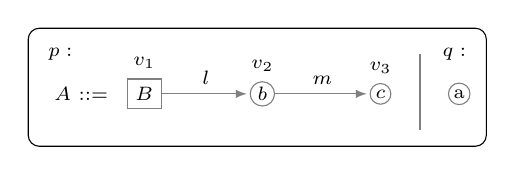
\begin{tikzpicture}[grammar]
	\node[rid] at (\ridX,\ridY) {$p:$};
	%The LHS
	\draw (\lhsX,0) node[lhs] (lhs) {$A$ ::=};
	
	%The RHS graph
	\draw (0.5,0) node[nont, label=90:$v_1$] (v1) {$B$};
	\draw (2,0) node[t, label=90:$v_2$] (v2) {$b$};
	\draw (3.5,0) node[t, label=90:$v_3$] (v3) {$c$};
	
	\draw[edge] (v1) -- (v2) node [edgeLabel] {$l$};
	\draw[edge] (v2) -- (v3) node [edgeLabel] {$m$};
	
	%The embedding
	%\draw node[w, label=0:$l;l;m$, label=-45:$a;b;c$] at (v1.south) (w-v1) {}
	%[wedge] (v1) -- (w-v1);
	
	%The next rule separator
	\draw[pipe] (4,\pipeBY) -- (4,\pipeUY);
	
	%The second RHS graph
	\node[rid] at (4.7,\ridY) {$q:$};
	\draw (4.5,0) node[t] (u1) {a};
	\end{tikzpicture}
\end{equation*}

Notice that, we use squares for non-terminal vertices, circles for terminal vertices, position the respective label inside the shape and the (possibly omitted) identifier over it. Over each edge is positioned its respective label. To depict the embedding function, we place near the respective vertex a small circle labeled with the image pairs of the embedding function for this node aligned vertically and separated by semi-colons, which in certain circumstances may also be omitted.

%TODO: comment on the different notation compared to the literature that uses attributed graphs and squares, etc... plus attributed graphs

%%%%%% Semantics %%%%%%
With these syntactic notions of the formalism presented, we introduce below its semantics by means of the concepts of derivation step, derivation and language.

\begin{definition}
	%TODO: Maybe define dstep more formally
	\label{def:gg_dstep}
	Let $GG = (\Sigma, \Delta, S, P)$ be a graph grammar and $G$ and $H$ be two graphs over $\Sigma$ that are disjoint to all right-hand sides from $P$, $G$ concretely derives in one step into $H$ with rule $r$ and vertex $v$, we write $G \cderiv{r}{v}{GG} H$ and call it a concrete derivation step, if, and only if, the following holds:
	\begin{align*}
		r & = (A \pro R, \omega) \in P \text{ and } A = \phi_G(v) \text{ and} \\
		V_H  & = (V_G \setminus \{v\}) \cup V_R \text{ and} \\
		E_H & = (E_G \setminus \{(w,l,t) \in E_G \st v = w \lor v = t\}) \\
		& \cup E_R \\
		& \cup \{(w,l,t) \st (w,l,v) \in E_G \land (l,\phi_G(w)) \in \omega(t)\} \\
		& \cup \{(t,l,w) \st (v,l,w) \in E_G \land (l,\phi_G(w)) \in \omega(t)\} \text{ and} \\
		\phi_H & = (\phi_G \setminus \{(v,x)\}) \cup \phi_R
	\end{align*}
	Notice that, without loss of generalization, we set $\omega(t) = \emptyset$ for all vertices $t$ without an image defined in $\omega$.
	
	If $G$ \textit{concretely derives} in one step into any graph $H'$ isomorphic to $H$, we say it \textit{derives} in one step into $H'$ and write $G \deriv{r}{v}{GG} H'$. 
	
	When $GG$, $r$ or $v$ are clear in the context or irrelevant we might omit them and simply write $G \cderiv{}{}{} H$ or $G \deriv{}{}{} H$. Moreover, we denote the reflexive transitive closure of $\deriv{}{}{}$ by $\derivtr{}{}{}$ and, for $G \derivtr{}{}{} H'$, we say $G$ derives in one or more steps into $H'$, or simply $G$ derives into $H'$.
\end{definition}

A concrete derivation can be informally understood as the replacement of a non-terminal vertex $v$ and all its adjacent edges in $G$ by a graph $R$ plus edges $e$ from former neighbors $w$ of $v$ to some vertices $t$ of $R$, provided $e$'s label and $w$'s label are in the embedding specification $\omega(t)$. That is, the embedding function $\omega$ of a rule specifies which neighbors of $v$ are to be connected with which vertices of $R$, according to their labels and the adjacent edges' labels. The process that governs the creation of these edges is called embedding and can occur in various forms in different graph grammar formalisms. We opted for a rather simple approach, in which the edges' directions and labels are maintained and cannot be used to define embedding. As an additional note, it is worth mentioning, that string grammars have no embedding because a replaced symbol in a string has ``connections" only with its left and right neighbors, so the replacement is always ``connected" with both sides.

\begin{definition}
	A derivation $D$ in $GG$ is a sequence of derivation steps and is written as
	\[ 
		D = (G_0 \deriv{r_0}{v_0}{} G_1 \deriv{r_1}{v_1}{} G_2 \deriv{r_2}{v_2}{} \dots \deriv{r_{n-1}}{v_{n-1}}{} G_n)
	\]
\end{definition}

\begin{definition}
	The language $L(GG)$ generated by the grammar $GG$ is the set of all graphs containing only terminal vertices derived from the start graph $\startG{GG}$, that is
	\[
		L(GG) = \{H \text{ is a graph over } \Delta \text{ and } \startG{GG} \derivtr{}{}{} H\}
	\]
\end{definition}

Notice that for every graph $G \in L(GG)$, there is at least one finite derivation $(\startG{GG} \deriv{r_0}{v_0}{} \dots \deriv{r_{n-1}}{v_{n-1}}{} G)$, but it is not guaranteed that this derivation be unique. In the case that there are more than one derivation for a $G$, we say that the grammar $GG$ is ambiguous.

Below we give one example of a grammar whose language consists of all chains of one or more vertices with interleaved vertices labeled with $a$ and $b$.

%Examples (chains)
\begin{example}{Chains of a's and b's.}
	$GG = (\{S,A,B,a,b,c\}, \{a,b,c\}, S, P)$, where $P$ is
	
		\noindent
	\begin{minipage}[t]{.27\textwidth}
		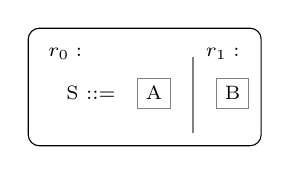
\begin{tikzpicture}[grammar]
		\node[rid] at (\ridX,\ridY) {$r_0:$};
		%The LHS
		\draw (\lhsX,0) node[lhs] (lhs) {S ::=};
		
		%The RHS graph
		\draw (0.5,0) node[nont] (v1) {A};
		
		%The next rule separator
		\draw[pipe] (1,-0.5) -- (1,\ridY);
		
		%The second RHS graph
		\node[rid] at (1.7,\ridY) {$r_1:$};
		\draw (1.5,0) node[nont] (v2) {B};
		\end{tikzpicture}
	\end{minipage}%
	\begin{minipage}[t]{.37\textwidth}
		\begin{tikzpicture}[grammar]
		\node[rid] at (\ridX,\ridY) {$r_2:$};
		%The LHS
		\draw (\lhsX,0) node[lhs] (lhs) {A ::=};
		
		%The RHS graph
		\draw (0.5,0) node[t] (v3) {a};
		\draw (1.5,0) node[nont] (v4) {B};
		
		\draw[edge] (v3) -- (v4) node [edgeLabel] {$c$};
		
		\draw node[w, label=0:$c$, label=-45:$b$] at (v3.south) (w-v3) {}
		[wedge] (v1) -- (w-v3);
		
		%The next rule separator
		\draw[pipe] (2,\pipeBY) -- (2,\pipeUY);
		
		%The second RHS graph
		\node[rid] at (2.7,\ridY) {$r_3:$};
		\draw (2.5,0) node[t] (v5) {a};
		\draw node[w, label=0:$c$, label=-45:$b$] at (v5.south) (w-v5) {}
		[wedge] (v5) -- (w-v5);
		\end{tikzpicture}
	\end{minipage}%
	\begin{minipage}[t]{.37\textwidth}
		\begin{tikzpicture}[grammar]
		\node[rid] at (\ridX,\ridY) {$r_4:$};
		%The LHS
		\draw (\lhsX,0) node[lhs] (lhs) {B ::=};
		
		%The RHS graph
		\draw (0.5,0) node[t] (v6) {b};
		\draw (1.5,0) node[nont] (v7) {A};
		
		\draw[edge] (v3) -- (v4) node [edgeLabel] {$c$};
		
		\draw node[w, label=0:$c$, label=-45:$a$] at (v6.south) (w-v6) {}
		[wedge] (v1) -- (w-v6);
		
		%The next rule separator
		\draw[pipe] (2,\pipeBY) -- (2,\pipeUY);
		
		%The second RHS graph
		\node[rid] at (2.7,\ridY) {$r_5:$};
		\draw (2.5,0) node[t] (v8) {b};
		\draw node[w, label=0:$c$, label=-45:$a$] at (v8.south) (w-v8) {}
		[wedge] (v8) -- (w-v8);
		\end{tikzpicture}
	\end{minipage}
	
	The graph $G=$
	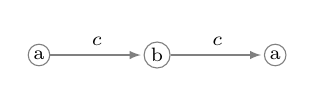
\begin{tikzpicture}[graph]
	\draw (0,0) node[t] (v1) {a};
	\draw (1.5,0) node[t] (v2) {b};
	\draw (3,0) node[t] (v3) {a};
	\draw[edge] (v1) -- (v2) node [edgeLabel] {$c$};
	\draw[edge] (v2) -- (v3) node [edgeLabel] {$c$};
	\end{tikzpicture}
	belongs to $L(GG)$ because it contains only terminal vertices and $\startG{GG}$ derives into it using the following derivation:
	\[
		\startG{GG} \deriv{r_0}{v_0}{} 
		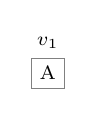
\begin{tikzpicture}[graph]
		\draw (0,0) node[nont, label=90:$v_1$] (v1) {A};
		\end{tikzpicture}
		\deriv{r_2}{v_1}{} 
		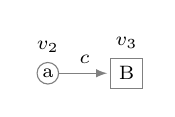
\begin{tikzpicture}[graph]
		\draw (1,0) node[t, label=90:$v_2$] (v2) {a};
		\draw (2,0) node[nont, label=90:$v_3$] (v3) {B};
		\draw[edge] (v2) -- (v3) node [edgeLabel] {$c$};
		\end{tikzpicture}
		\deriv{r_4}{v_3}{}
		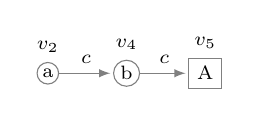
\begin{tikzpicture}[graph]
		\draw (1,0) node[t, label=90:$v_2$] (v2) {a};
		\draw (2,0) node[t, label=90:$v_4$] (v4) {b};
		\draw (3,0) node[nont, label=90:$v_5$] (v5) {A};
		\draw[edge] (v2) -- (v4) node [edgeLabel] {$c$};
		\draw[edge] (v4) -- (v5) node [edgeLabel] {$c$};
		\end{tikzpicture}
		\deriv{r_3}{v_5}{}
		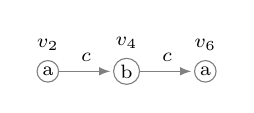
\begin{tikzpicture}[graph]
		\draw (0,0) node[t, label=90:$v_2$] (v2) {a};
		\draw (1,0) node[t, label=90:$v_4$] (v4) {b};
		\draw (2,0) node[t, label=90:$v_6$] (v6) {a};
		\draw[edge] (v2) -- (v4) node [edgeLabel] {$c$};
		\draw[edge] (v4) -- (v6) node [edgeLabel] {$c$};
		\end{tikzpicture}
	\]
\end{example}

%TODO: Church-Rosser theorem??

%%%==================================================================%%%
%%%%%%%%%%%%%%%%%%%% TRIPLE GRAPH GRAMMARS %%%%%%%%%%%%%%%%%%%%%%%%%%%%%
%%%==================================================================%%%
\subsection{Triple Graph Grammars}
Building upon the concepts of graphs and graph grammars, we present, in the following, our understanding over triple graphs and triple graph grammars (TGGs), supported by the TGG specification from \cite{schurr1994specification}.

%%%%%% Syntax %%%%%%

\begin{definition}
	A directed labeled triple graph $TG = G_s \ms{m_s} G_c \mt{m_t} G_t$ over $\Sigma$ consists of three disjoint directed labeled graphs over $\Sigma$ (see \ref{def:graph}), respectively, the source graph $G_s$, the correspondence graph $G_c$ and the target graph $G_t$, together with two injective morphisms (see \ref{def:morphism}) $m_s: V_{G_c} \to V_{G_s}$ and $m_t : V_{G_c} \to G_{G_t}$. Directed labeled triple graphs are often referred to simply as triple graphs and we might omit the morphisms' names in the notation. Moreover, we denote the set of all triple graphs over $\Sigma$ as $\alltgraphs{\Sigma}$. We might refer to all vertices of $TG$ by $V_{TG}:= V_s \cup V_c \cup V_t$, all edges by $E_{TG}:= E_s \cup E_c \cup E_t$ and the complete labeling function by $\phi_{TG}:= \phi_{G_s} \cup \phi_{G_c} \cup \phi_{G_t}$.
	%TODO: Do we need empty triple graph?
\end{definition}

\begin{definition}
	A $\Gamma\text{-boundary}$ triple graph $TG = G_s \ms{} G_c \mt{} G_t$ is such that $G_s$, $G_c$ and $G_t$ are $\Gamma\text{-boundary}$ graphs.
\end{definition}

%TODO: Make sure introduction says something about triple graphs
As stated before, triple graphs are for us a good tool to express relations between the vertices of two graphs. In the context of model transformation, where graphs represent models, a triple graph holds, for example, a source model and a target model generated from the source, together with the relationship between their vertices. We also advise that in literature, TGGs are often modeled as typed graphs, but we judge that for our circumstance labeled graphs fit better and we are convinced that such divergence does not threat the validity of our approach.

Below we start introducing the standard definition of TGG of the current research's literature. As the reader should notice, this definition of TGG does not fit our needs optimally, because it defines a context-sensitive-like graph grammar whilst we wish a context-free-like graph grammar to use together with the NCE graph grammar formalism. Hence, after presenting the conventional TGG definition, we refine it to create a NCE TGG, that fits our context best.

\begin{definition}
	\label{def:stgg}
	A triple graph grammar $TGG = (\Sigma, \Delta \subseteq \Sigma, S \in \Sigma, P)$ consists of, analogously to graph grammars (see \ref{def:gg}), an alphabet $\Sigma$, a set of terminal symbols $\Delta$ (also define $\Gamma := \Sigma \setminus \Delta$), a start symbol $S$ and a set of production rules $P$ of the form $L \pro R$ with $L = L_s \ms{} L_c \mt{} L_t$ and $R = R_s \ms{} R_c \mt{} R_t$ and $L \subseteq R.$
\end{definition}

\begin{definition}
	A triple graph grammar with neighborhood-controlled embedding (NCE TGG) $TGG = (\Sigma, \Delta \subseteq \Sigma, S \in \Sigma, P)$ consists of, an alphabet $\Sigma$, a set of terminal symbols $\Delta$ (also define $\Gamma := \Sigma \setminus \Delta$), a start symbol $S$ and a set of production rules $P$ of the form $(A \pro (R_s \ms{} R_c \mt{} R_t), \omega_s, \omega_t)$ with $A \in \Gamma$ being the left-hand side, $(R_s \ms{} R_c \mt{} R_t) \in \alltgraphs{\Sigma}$ the right-hand side and $\omega_s : V_{R_s} \pto 2^{\Sigma \times \Sigma}$ and $\omega_t : V_{R_t} \pto 2^{\Sigma \times \Sigma}$ the partial embedding functions from the right-hand side's vertices to pairs of edge and label symbols. We might refer to the complete embedding function by $\omega:= \omega_s \cup \omega_t$.
	
	For convenience, define the start triple graph of $TGG$ as $\startTG{TGG} := Z_s \ms{ms} Z_c \mt{mt} Z_t$ where $Z_s = (\{s_0\},\emptyset,\{s_0 \mapsto S\})$, $Z_c = (\{c_0\},\emptyset,\{c_0 \mapsto S\})$, $Z_t = (\{t_0\},\emptyset,\{t_0 \mapsto S\})$, $ms = \{c_0 \mapsto s_0 \}$ and $mt = \{c_0 \mapsto t_0 \}$.
	
	%TODO: Extend here with look-ahead
	%TODO: discuss empty productions(?)
	
	%TODO: mabe use format S \pro Gs .... without three symbols in the lhs
\end{definition}

\begin{definition}
	A boundary triple graph grammar with neighborhood-controlled embedding (BNCE TGG) is such that non-terminal vertices of the right-hand sides of rules are not neighbors. That is, the triple graph grammar $TGG$ is boundary iff all its rules' right-hand sides are $\Gamma\text{-boundary}$ triple graphs.
\end{definition}

The most important difference between the traditional TGG and the NCE TGG, is that the former allows any triple graph to occur in the left-hand sides, whereas the latter only one symbol. In addition to that, traditional TGG requires that the whole left hand side occur also in the right-hand side, that is to say, the rules are monotonic crescent. Therewith, embedding is not an issue, because an occurrence of the left-hand side is not effectively replaced by the right-hand side, instead, only new vertices are added. On the other hand, NCE TGG has to deal with embedding through the embedding function.

%%%%%% Semantics %%%%%%
In the following, the semantics for NCE TGG is presented analogously to the semantics for NCE graph grammars.

\begin{definition}
	%TODO: Maybe define dstep more formally
	\label{def:tgg_dstep}
	Let $TGG = (\Sigma, \Delta, S, P)$ be a NCE TGG and $G = G_s \ms{g_s} G_c \mt{g_t} G_t$ and $H = H_s \ms{h_s} H_c \mt{h_t} H_t$ be two triple graphs over $\Sigma$ disjoint from any right-hand side from $P$, $G$ concretely derives in one step into $H$ with rule $r$ and distinct vertices $v_s, v_c, v_t$, we write $G \tcderiv{r}{v_s,v_c,v_t}{TGG} H$ if, and only if, the following holds:
	\begin{align*}
		r & = (A \pro (R_s \ms{r_s} R_c \mt{r_t} R_t), \omega_s, \omega_t) \in P \text{ and } \\
		A & = \phi_{G_s}(v_s) = \phi_{G_c}(v_c) = \phi_{G_t}(v_t) \text{ and}\\
		V_{H_s}  & = (V_{G_s} \setminus \{v_s\}) \cup V_{R_s} \text{ and}\\
		V_{H_c}  & = (V_{G_c} \setminus \{v_c\}) \cup V_{R_c} \text{ and}\\
		V_{H_t}  & = (V_{G_t} \setminus \{v_t\}) \cup V_{R_t} \text{ and}\\
		E_{H_s} & = (E_{G_s} \setminus \{(w,l,t) \in E_{G_s} \st w \in \{v_s\} \lor t \in \{v_s\} \}) \cup E_{R_s} \\
		& \cup \{(w,l,t) \st (w,l,v) \in E_{G_s} \land (l,\phi_{G_s}(w)) \in \omega_{s}(t)\} \\
		& \cup \{(t,l,w) \st (v,l,w) \in E_{G_s} \land (l,\phi_{G_s}(w)) \in \omega_{s}(t)\} \text{ and} \\
		E_{H_c} & = (E_{G_c} \setminus \{(w,l,t) \in E_{G_c} \st w = v_c \lor t = v_c \}) \cup E_{R_c} \text{ and} \\
		E_{H_t} & = (E_{G_t} \setminus \{(w,l,t) \in E_{G_t} \st w = v_t \lor t = v_t \}) \cup E_{R_t} \\
		& \cup \{(w,l,t) \st (w,l,v) \in E_{G_t} \land (l,\phi_{G_t}(w)) \in \omega_{t}(t)\} \\
		& \cup \{(t,l,w) \st (v,l,w) \in E_{G_t} \land (l,\phi_{G_t}(w)) \in \omega_{t}(t)\} \text{ and} \\
		h_s		& = (g_s \setminus \{(v_c,x)\}) \cup r_s  \\
		h_t		& = (g_t \setminus \{(v_c,x)\}) \cup r_t  \\
		\phi_{H_s} & = (\phi_{G_s} \setminus \{(v_s,x)\}) \cup \phi_{R_s} \text{ and}\\
		\phi_{H_c} & = (\phi_{G_c} \setminus \{(v_c,x)\}) \cup \phi_{R_c} \text{ and}\\
		\phi_{H_t} & = (\phi_{G_t} \setminus \{(v_t,x)\}) \cup \phi_{R_t}\\
	\end{align*}
	Notice that, without loss of generalization, we set $\omega(t) = \emptyset$ for all vertices $t$ without an image defined in $\omega$.
	
	Analogously to graph grammars, if $G \cderiv{r}{v_s,v_c,v_t}{TGG} H$ and $H' \in [H]$, then $G \tderiv{r}{v_s,v_c,v_t}{TGG} H'$, moreover the reflexive transitive closure of $\tderiv{}{}{}$ is denoted by $\tderivtr{}{}{}$ and we call these relations by the same names as before, namely, derivation in one step and derivation. We might also omit identifiers.
\end{definition}

A concrete derivation of a triple graph $G = G_s \ms{g_s} G_c \mt{g_t} G_t$ can de informally understood as concrete derivations (see \ref{def:gg_dstep}) of $G_s$, $G_c$ and $G_t$ according to the right-hand sides $R_s$, $R_c$ and $R_t$. The only remark is the absence of an embedding mechanism for the correspondence graph, which edges are not important for our application. Nevertheless, the addition of such a mechanism for the correspondence graph should not be a problem if it is desired.

\begin{definition}
	A derivation $D$ in $TGG$ is a sequence of derivation steps
	\[ 
	D = (G_0 \tderiv{r_0}{s_0,c_0,t_0}{} G_1 \tderiv{r_1}{s_1,c_1,t_1}{} G_2 \tderiv{r_2}{s_2,c_2,t_2}{} \dots \tderiv{r_{n-1}}{s_{n-1},c_{n-1},t_{n-1}}{} G_n)
	\]
\end{definition}

\begin{definition}
	\label{def:tlanguage}
	The language $L(TGG)$ generated by the triple grammar $TGG$ is the set of all triple graphs containing only terminal vertices derived from the start triple graph $\startTG{TGG}$, that is
	\[
	L(TGG) = \{H \text{ is a triple graph over } \Delta \text{ and } \startTG{TGG} \tderivtr{}{}{} H\}
	\]
\end{definition}

Our concrete syntax for NCE TGG is similar to the one for NCE graph grammars and is presented below by means of the Example \ref{ex:pseudocode2controlflow}. The only difference is at the right-hand sides, that include the morphisms between the correspondence graph and source and target graphs depicted with dashed lines.

%Concrete syntax and examples (Pseudocode 2 Control Flow [sourcecode2controlflow])
\begin{example}{Pseudocode to Controlflow.}
	\label{ex:pseudocode2controlflow}
	%TODO: So far, it should be let clear what TGGs are used for (introduction)
	This example illustrates the definition of a BNCE TGG that characterizes the language of all $Pseudocode$ graphs together with their respective $Controlflow$ graphs. A $Pseudocode$ graph is an abstract representation of a program written in a pseudo-code where vertices refer to \textit{actions}, \textit{ifs} or \textit{whiles} and edges connect these items together according to how they appear in the program. A $Controlflow$ graph is a more abstract representation of a program, where vertices can only be either a \textit{command} or a \textit{branch}.
	
	Consider, for instance, the program $main$ below on the left, written in a pseudo-code. The triple graph $TG$ on the right consists of the $Pseudocode$ graph of $main$ connected to the $Controlflow$ graph of the same program through the correspondence graph in the middle of them. In such graph, the vertex labels of the $Pseudocode$ graph $p, i, a, w$ correspond to the concepts of \textit{program}, \textit{if}, \textit{action} and \textit{while}, respectively. The edge label $f$ is given to the edge from the vertex $p$ to the program's first statement, $x$ stands for \textit{next} and indicates that a statement is followed by another, $p$ and $n$ stand for \textit{positive} and \textit{negative} and indicate which assignments correspond to the positive of negative case of the \textit{if}'s evaluation, finally $l$ stands for \textit{last} and indicates the last action of a loop. In the $Controlflow$ graph, the vertex labels $g, b, c$ stand for the concepts of \textit{graph}, \textit{branch} and \textit{command}, respectively. The edge label $r$ is given to the edge from the vertex $g$ to the first program's statement, $x, p$ and $n$ mean, analogous to the former graph, \textit{next}, \textit{positive} and \textit{negative}. In the correspondence graph, the labels $pg, ib, ac, wb$ serve to indicate which labels in the source and target graphs are being connected through the triple graph's morphism.
	
	\begin{minipage}[h]{.48\textwidth}
	\begin{algorithmic}[!ht]
		\State \Program $main(n)$
		\If {$n < 0$}
			\State \Return $\Nothing$
		\Else
			\State $f \gets 1$ 
			\While {$n > 0$}
				\State $f \gets f * n$
				\State $n \gets n - 1$
			\EndWhile
			\State \Return $\Just f$
		\EndIf
	\end{algorithmic}
\end{minipage}
\begin{minipage}[h]{.5\textwidth}
	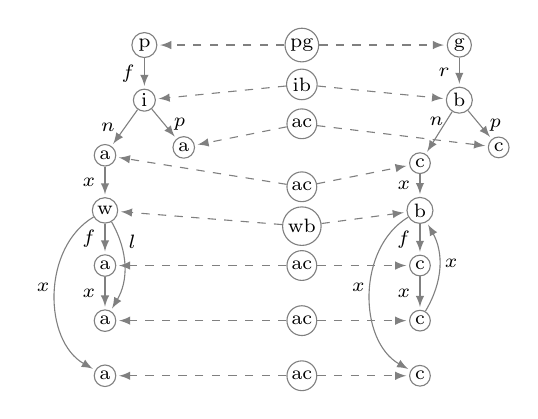
\begin{tikzpicture}[graph]
	\draw (1,0) node[t] (s1) {p};
	\draw (1,-0.7) node[t] (s2) {i};
	\draw (1.5,-1.3) node[t] (s3) {a};
	\draw (0.5,-1.4) node[t] (s4) {a};
	\draw (0.5,-2.1) node[t] (s5) {w};
	\draw (0.5,-2.8) node[t] (s6) {a};
	\draw (0.5,-3.5) node[t] (s7) {a};
	\draw (0.5,-4.2) node[t] (s8) {a};
	
	\draw[edge] (s1) -- (s2) node [vledgeLabel] {$f$};
	\draw[edge] (s2) -- (s3) node [vredgeLabel] {$p$};
	\draw[edge] (s2) -- (s4) node [vledgeLabel] {$n$};
	\draw[edge] (s4) -- (s5) node [vledgeLabel] {$x$};
	\draw[edge] (s5) -- (s6) node [vledgeLabel] {$f$};
	\draw[edge] (s5) to [bend left] (s7) node [above=25pt, right=3pt] {$l$};
	\draw[edge] (s5) to [bend right=60] (s8) node [above=30pt, left=13pt] {$x$};
	\draw[edge] (s6) -- (s7) node [vledgeLabel] {$x$};
	%
	\draw (3,0) node[t] (c1) {pg};
	\draw (3,-0.5) node[t] (c2) {ib};
	\draw (3,-1.0) node[t] (c3) {ac};
	\draw (3,-1.8) node[t] (c4) {ac};
	\draw (3,-2.3) node[t] (c5) {wb};
	\draw (3,-2.8) node[t] (c6) {ac};
	\draw (3,-3.5) node[t] (c7) {ac};
	\draw (3,-4.2) node[t] (c8) {ac};
	%
	\draw (5,0) node[t] (t1) {g};
	\draw (5,-0.7) node[t] (t2) {b};
	\draw (5.5,-1.3) node[t] (t3) {c};
	\draw (4.5,-1.5) node[t] (t4) {c};
	\draw (4.5,-2.1) node[t] (t5) {b};
	\draw (4.5,-2.8) node[t] (t6) {c};
	\draw (4.5,-3.5) node[t] (t7) {c};
	\draw (4.5,-4.2) node[t] (t8) {c};
	
	\draw[edge] (t1) -- (t2) node [vledgeLabel] {$r$};
	\draw[edge] (t2) -- (t3) node [vredgeLabel] {$p$};
	\draw[edge] (t2) -- (t4) node [above=15pt, right=0pt] {$n$};
	\draw[edge] (t4) -- (t5) node [vledgeLabel] {$x$};
	\draw[edge] (t5) -- (t6) node [vledgeLabel] {$f$};
	\draw[edge] (t7) to [bend right] (t5) node [below=15pt, right=3pt] {$x$};
	\draw[edge] (t5) to [bend right=60] (t8) node [above=30pt, left=13pt] {$x$};
	\draw[edge] (t6) -- (t7) node [vledgeLabel] {$x$};
	%
	\draw[morph] (c1) -- (s1);
	\draw[morph] (c1) -- (t1);
	\draw[morph] (c2) -- (s2);
	\draw[morph] (c2) -- (t2);
	\draw[morph] (c3) -- (s3);
	\draw[morph] (c3) -- (t3);
	\draw[morph] (c4) -- (s4);
	\draw[morph] (c4) -- (t4);
	\draw[morph] (c5) -- (s5);
	\draw[morph] (c5) -- (t5);
	\draw[morph] (c6) -- (s6);
	\draw[morph] (c6) -- (t6);
	\draw[morph] (c7) -- (s7);
	\draw[morph] (c7) -- (t7);
	\draw[morph] (c8) -- (s8);
	\draw[morph] (c8) -- (t8);
	\end{tikzpicture}
\end{minipage}%
	
	The main difference between the two graphs is the absence of the $w$ label in the $Controlflow$ graph, what makes it encode loops through the combination of $b$-labeled vertices and $x$-labeled edges.
	
	The TGG that specifies the relation between these two types of graphs is $TGG = (\{S, A, p, a, i, w, g, b, c, f, x, p, n, l, r, pg, ac, ib, wb\}, \{p, a, i, w, g, b, c, f, x, p, n, l, r, pg, ac, ib, wb\}, S, P)$, where $P$ is
	
		\noindent
	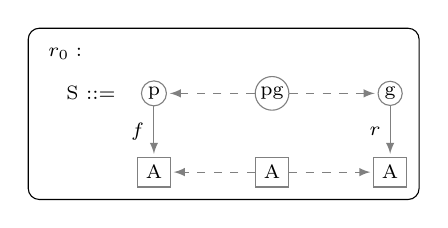
\begin{tikzpicture}[grammar]
	\node[rid] at (\ridX,\ridY) {$r_0:$};
	\draw (\lhsX,0) node[lhs] (lhs) {S ::=};
	
	\draw (0.5,0) node[t] (s1) {p};
	\draw (0.5,-1) node[nont] (s2) {A};
	\draw[edge] (s1) -- (s2) node [vledgeLabel] {$f$};
	%%
	\draw (2,0) node[t] (c1) {pg};
	\draw (2,-1) node[nont] (c2) {A};
	%%
	\draw (3.5,0) node[t] (t1) {g};
	\draw (3.5,-1) node[nont] (t2) {A};
	\draw[edge] (t1) -- (t2) node [vledgeLabel] {$r$};
	%%
	\draw[morph] (c1) -- (s1);
	\draw[morph] (c1) -- (t1);
	\draw[morph] (c2) -- (s2);
	\draw[morph] (c2) -- (t2);
	\end{tikzpicture}
	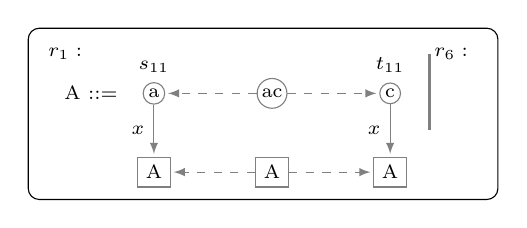
\begin{tikzpicture}[grammar]
	\node[rid] at (\ridX,\ridY) {$r_1:$};
	\draw (\lhsX,0) node[lhs] (lhs) {A ::=};
	
	\draw (0.5,0) node[t, label=90:$s_{11}$] (s1) {a};
	\draw (0.5,-1) node[nont] (s2) {A};
	\draw[edge] (s1) -- (s2) node [vledgeLabel] {$x$};
	%\draw node[uw] at (s1.east) (w-s1) {} [wedge] (s1) -- (w-s1);
	%%
	\draw (2,0) node[t] (c1) {ac};
	\draw (2,-1) node[nont] (c2) {A};
	%%
	\draw (3.5,0) node[t, label=90:$t_{11}$] (t1) {c};
	\draw (3.5,-1) node[nont] (t2) {A};
	\draw[edge] (t1) -- (t2) node [vledgeLabel] {$x$};
	%\draw node[uw] at (t1.north) (w-t1) {} [wedge] (t1) -- (w-t1);
	%%
	\draw[morph] (c1) -- (s1);
	\draw[morph] (c1) -- (t1);
	\draw[morph] (c2) -- (s2);
	\draw[morph] (c2) -- (t2);
	
	%%%%
	\draw[pipe] (4,\pipeBY) -- (4,\pipeUY);
	
	\node[rid] at (4.6,\ridY) {$r_6:$};
	\draw (4.6,0) node[empty] (s3) {$\emptyGraph$};
	\end{tikzpicture}
	
	\noindent
	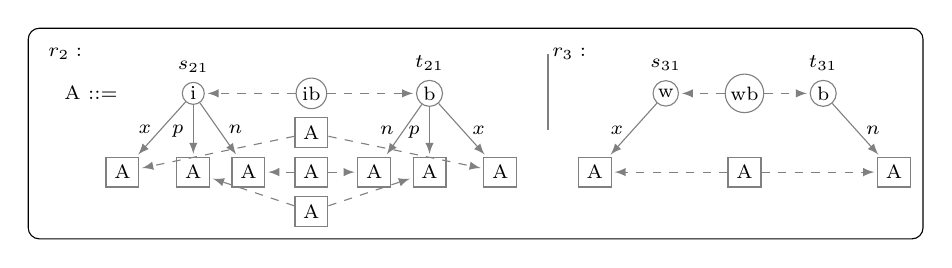
\begin{tikzpicture}[grammar]
	\node[rid] at (\ridX,\ridY) {$r_2:$};
	\draw (\lhsX,0) node[lhs] (lhs) {A ::=};
	
	\draw (1,0) node[t, label=90:$s_{21}$] (s1) {i};
	\draw (0.1,-1) node[nont] (s2) {A};
	\draw (1,-1) node[nont] (s3) {A};
	\draw (1.7,-1) node[nont] (s4) {A};
	\draw[edge] (s1) -- (s2) node [vledgeLabel] {$x$};
	\draw[edge] (s1) -- (s3) node [vledgeLabel] {$p$};
	\draw[edge] (s1) -- (s4) node [vredgeLabel] {$n$};
	%\draw node[uw] at (s1.north) (w-s1) {} [wedge] (s1) -- (w-s1);
	%%
	\draw (2.5,0) node[t] (c1) {ib};
	\draw (2.5,-0.5) node[nont] (c2) {A};
	\draw (2.5,-1) node[nont] (c4) {A};
	\draw (2.5,-1.5) node[nont] (c3) {A};
	%%
	\draw (4,0) node[t, label=90:$t_{21}$] (t1) {b};
	\draw (3.3,-1) node[nont] (t4) {A};
	\draw (4,-1) node[nont] (t3) {A};
	\draw (4.9,-1) node[nont] (t2) {A};
	\draw[edge] (t1) -- (t4) node [vledgeLabel] {$n$};
	\draw[edge] (t1) -- (t3) node [vledgeLabel] {$p$};
	\draw[edge] (t1) -- (t2) node [vredgeLabel] {$x$};
	%\draw node[uw] at (t1.north) (w-t1) {} [wedge] (t1) -- (w-t1);
	%%
	\draw[morph] (c1) -- (s1);
	\draw[morph] (c1) -- (t1);
	\draw[morph] (c2) -- (s2);
	\draw[morph] (c2) -- (t2);
	\draw[morph] (c3) -- (s3);
	\draw[morph] (c3) -- (t3);
	\draw[morph] (c4) -- (s4);
	\draw[morph] (c4) -- (t4);
	
	%%%%
	\draw[pipe] (5.5,\pipeBY) -- (5.5,\pipeUY);
	
	\node[rid] at (6.1,\ridY) {$r_3:$};
	
	\draw (7,0) node[t, label=90:$s_{31}$] (s5) {w};
	\draw (6.1,-1) node[nont] (s6) {A};
	\draw[edge] (s5) -- (s6) node [vledgeLabel] {$x$};
	%\draw node[uw] at (s5.north) (w-s5) {} [wedge] (s5) -- (w-s5);
	%%
	\draw (8,0) node[t] (c5) {wb};
	\draw (8,-1) node[nont] (c6) {A};
	%%
	\draw (9,0) node[t, label=90:$t_{31}$] (t5) {b};
	\draw (9.9,-1) node[nont] (t6) {A};
	\draw[edge] (t5) -- (t6) node [vredgeLabel] {$n$};
	%\draw node[uw] at (t5.north) (w-t5) {} [wedge] (t5) -- (w-t5);
	%%
	\draw[morph] (c5) -- (s5);
	\draw[morph] (c5) -- (t5);
	\draw[morph] (c6) -- (s6);
	\draw[morph] (c6) -- (t6);
	\end{tikzpicture}
	
	\noindent
	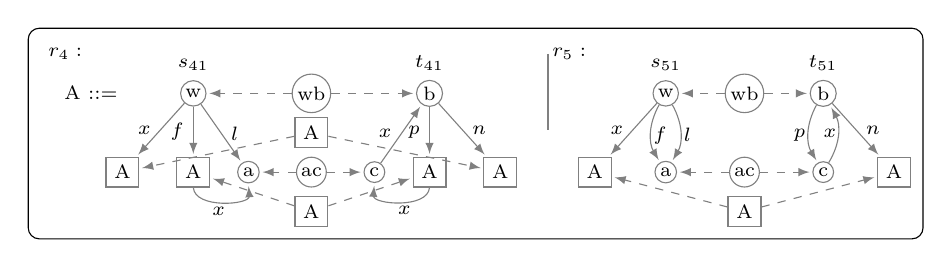
\begin{tikzpicture}[grammar]
	\node[rid] at (\ridX,\ridY) {$r_4:$};
	\draw (\lhsX,0) node[lhs] (lhs) {A ::=};
	
	\draw (1,0) node[t, label=90:$s_{41}$] (s1) {w};
	\draw (0.1,-1) node[nont] (s2) {A};
	\draw (1,-1) node[nont] (s3) {A};
	\draw (1.7,-1) node[t] (s4) {a};
	
	\draw[edge] (s1) -- (s2) node [vledgeLabel] {$x$};
	\draw[edge] (s1) -- (s3) node [vledgeLabel] {$f$};
	\draw[edge] (s3) to [bend right=90] (s4) node [below=10pt, left=5pt] {$x$};
	\draw[edge] (s1) -- (s4) node [vredgeLabel] {$l$};
	%\draw node[uw] at (s1.north) (w-s1) {} [wedge] (s1) -- (w-s1);
	%%
	\draw (2.5,0) node[t] (c1) {wb};
	\draw (2.5,-0.5) node[nont] (c2) {A};
	\draw (2.5,-1) node[t] (c4) {ac};
	\draw (2.5,-1.5) node[nont] (c3) {A};
	%%
	\draw (4,0) node[t, label=90:$t_{41}$] (t1) {b};
	\draw (3.3,-1) node[t] (t4) {c};
	\draw (4,-1) node[nont] (t3) {A};
	\draw (4.9,-1) node[nont] (t2) {A};
	\draw[edge] (t1) -- (t2) node [vredgeLabel] {$n$};
	\draw[edge] (t1) -- (t3) node [vledgeLabel] {$p$};
	\draw[edge] (t3) to [bend left=90] (t4) node [below=10pt, right=5pt] {$x$};
	\draw[edge] (t4) -- (t1) node [vledgeLabel] {$x$};
	%\draw node[uw] at (t1.north) (w-t1) {} [wedge] (t1) -- (w-t1);
	%%
	\draw[morph] (c1) -- (s1);
	\draw[morph] (c1) -- (t1);
	\draw[morph] (c2) -- (s2);
	\draw[morph] (c2) -- (t2);
	\draw[morph] (c3) -- (s3);
	\draw[morph] (c3) -- (t3);
	\draw[morph] (c4) -- (s4);
	\draw[morph] (c4) -- (t4);
	
	%%%%
	\draw[pipe] (5.5,\pipeBY) -- (5.5,\pipeUY);
	
	\node[rid] at (6.1,\ridY) {$r_5:$};
	
	\draw (7,0) node[t, label=90:$s_{51}$] (s5) {w};
	\draw (6.1,-1) node[nont] (s6) {A};
	\draw (7,-1) node[t] (s7) {a};
	\draw[edge] (s5) -- (s6) node [vledgeLabel] {$x$};
	\draw[edge] (s5) to [bend right] (s7) node [vbedgeLabel] {$f$};
	\draw[edge] (s5) to [bend left] (s7) node [above=10pt, right=1pt] {$l$};
	%\draw node[uw] at (s5.north) (w-s5) {} [wedge] (s5) -- (w-s5);
	%%
	\draw (8,0) node[t] (c5) {wb};
	\draw (8,-1.5) node[nont] (c6) {A};
	\draw (8,-1) node[t] (c7) {ac};
	%%
	\draw (9,0) node[t, label=90:$t_{51}$] (t5) {b};
	\draw (9,-1) node[t] (t7) {c};
	\draw (9.9,-1) node[nont] (t6) {A};
	\draw[edge] (t5) -- (t6) node [vredgeLabel] {$n$};
	\draw[edge] (t5) to [bend right] (t7) node [above=10pt, left=1pt] {$p$};
	\draw[edge] (t7) to [bend right] (t5) node [below=5pt] {$x$};
	%\draw node[uw] at (t5.north) (w-t5) {} [wedge] (t5) -- (w-t5);
	%%
	\draw[morph] (c5) -- (s5);
	\draw[morph] (c5) -- (t5);
	\draw[morph] (c6) -- (s6);
	\draw[morph] (c6) -- (t6);
	\draw[morph] (c7) -- (s7);
	\draw[morph] (c7) -- (t7);
	\end{tikzpicture}
	
	\noindent
	with $\sigma_1(s_{11}) = \sigma_2(s_{21}) = \sigma_3(s_{31}) = \sigma_4(s_{41}) =\sigma_5(s_{51}) = \{ (f,p), (x,a), (x,i),$ $ (x,w), (p,i), (n,i), (l,w), (f,w) \}$ and $\tau_1(t_{11}) = \tau_2(t_{21}) = \tau_3(t_{31}) = \tau_4(t_{41}) =\tau_5(t_{51}) = \{ (r,g), (x,c), (x,b), (p,b), (n,b)\}$ being the complete definition of the source and target embedding functions of the rules, respectively.
	
	The rule $r_0$ relates programs to graphs, $r_1$ actions to commands, $r_2$ ifs to branches, $r_3$ empty whiles to simple branches, $r_4$ filled whiles to filled loops with branches, $r_5$ whiles with one action to loops with branches with one command and, finally, $r_6$ produces an empty graph from a symbol $A$, what allows any derivation in the grammar to finish.
	
	The aforementioned triple graph $TG$ is in $L(TGG)$, because the derivation
	$
	\startTG{TGG} \tderiv{r_0}{}{} G_1 \tderiv{r_2}{}{} G_2 \tderiv{r_6}{}{} G_3 \tderiv{r_1}{}{} G_4 \tderiv{r_6}{}{} G_5 \tderiv{r_1}{}{} G_6 \tderiv{r_4}{}{} G_7 \tderiv{r_1}{}{} G_8 \tderiv{r_6}{}{} G_9 \tderiv{r_1}{}{} G_{10} \tderiv{r_6}{}{} TG
	$
	is a derivation in TGG with appropriate $G_i$ for $1 \le i \le 10$.
\end{example}

%%%%%%%%%%%%%%%%%%%%%%%%%%%%%%%%%%%%%%%%%%%%%%%%%%%%%%%%%%%%%%%%%%%%%%%%
%%%%%%%%%%%%%%%%%%%%%%%%%%%%%% PARSING %%%%%%%%%%%%%%%%%%%%%%%%%%%%%%%%%
%%%%%%%%%%%%%%%%%%%%%%%%%%%%%%%%%%%%%%%%%%%%%%%%%%%%%%%%%%%%%%%%%%%%%%%%
\section{Parsing of Graphs with BNCE Graph Grammars}
In the last section we cleared how the concepts of graphs and languages fit together. In this section we are interested in the problem of deciding, given a BNCE graph grammar $GG$ and a graph $G$, whether $G \in L(GG)$. This is sometimes called the \textit{membership} problem and can be solved through a recognizer algorithm that always finishes answering yes if and only if $G \in L(GG)$ and no otherwise. A slight extension of this problem is the \textit{parsing} problem, which consists of deciding if $G \in L(GG)$ and finding a derivation $\startG{GG} \derivtr{}{}{} G$.

%TODO: The practical use of it: model checking... model validation

The parsing algorithm posed in this section is an imperative view of the method proposed by ()%TODO: cite 27
, which is basically a version fro graphs of the well-known CYK (Cocke-Young-Kassami) algorithm for parsing of strings with a context-free (string) grammar. Preliminarily to the actual algorithm's presentation, we introduce some necessary concepts that are used by it. The first of them is the neighborhood preserving normal form.

\begin{definition}
	\label{def:np}
	A BNCE graph grammar $GG = (\Sigma, \Delta, S, P)$ is neighborhood preserving (NP), if and only if, the embedding of each rule with left-hand side $A$ is greater or equal than the context of each $A$-labeled vertex in the grammar. That is, let 
	\[\cont{(A \pro R,\omega)}{v} =\{(l,\phi_{R}(w)) \st (v,l,w) \in E_R \text { or } (w,l,v) \in E_R \} \cup \omega(v) \]
	be the context of $v$ in the rule $(A \pro R,\omega)$ and
	\[\scont{GG}{A} = \bigcup_{(B \pro Q,\zeta) \in P, v \in V_Q, \phi_Q(v) = A} \cont{B \pro Q,\zeta}{v} \] 
	be the context of the symbol $A$ in the grammar $GG$, then $GG$ is a NP BNCE graph grammar, if and only if,
	\[ \forall r = (A \pro R,\omega) \in P \. \scont{GG}{A} \subseteq \bigcup_{v \ in V_R} \omega(v) \]
\end{definition}

The NP property is important to the correctness of the parsing algorithm. Furthermore, it is guaranteed that any BNCE graph grammar can be transformed in an equivalent NP BNCE graph grammar in polynomial time. More details in () %TODO: cite 27

The next paragraphs present zone vertices and zone graphs, that are our understanding of the concepts also from %TODO: cite 27

\begin{definition}
	A zone vertex $h$ of a graph $G$ over $\Sigma$ is a pair $(\sigma \in \Sigma, U \subseteq V_G)$, that is, a symbol from $\Sigma$ and a subset of the vertices of $G$.
	
	A zone vertex can be understood as a contraction of a subgraph of $G$ defined by the vertices $U$ into one vertex with symbol $\sigma$.
\end{definition}

\begin{definition}
	Let $H = \{(\sigma_0,U_0),(\sigma_1,U_1),\dots,(\sigma_m,U_m)\}$ be a set of zone vertices of a graph $G$ over $\Sigma$ with disjoint vertices (i.e. $U_i \cap U_j = \emptyset$ for all $0 \leq i,j \leq m \text{ and } i \neq j$) and $V(H) = \bigcup_{0 \leq i \leq m}{U_i}$. A zone graph $Z(H)$ for $H$ is $Z(H) = (V, E, \phi)$ with $V$ being the zone vertices, $E \subseteq V \times \Sigma \times V$ the edges between zone vertices and $\phi: V \to \Sigma$ the labeling function, determined by
	\begin{align*}
		V & = H \cup \{(\phi_G(x),\{x\}) \st x \in neigh_G(V(H)) \}\\
		E & = \{((\sigma,U),l,(\eta,T)) \st (\sigma,U),(\eta,T) \in V \text{ and } U \neq T \text{ and } \\
		& (u,l,t) \in E_G \text{ and } u \in U \text{ and } t \in T\} \\
		\phi & = \{(\sigma,U) \mapsto \sigma\}
	\end{align*}
	The zone graph $Z(H)$ can be intuitively understood as a subgraph of $G$, where each zone vertex in $V_{Z(H)}$ is either a $(\sigma_i,U_i)$ of $H$, which is a contraction of the vertices $U_i$ of $G$, or a $(\phi_G(x),\{x\})$, which stems from $x$ being a neighbor of some vertex in $V_i$.
	
	For convenience, define $Y(H)$ as the subgraph of $Z(H)$ induced by H.
	%TODO: maybe write more about induction
	%TODO: comment about information duplication of labels
\end{definition}

\begin{definition}
	Let $h$ be a zone vertex, $r$ a production rule and $X$ a (potentially empty) set of parsing trees, $\ptree{h}{r}{X}$ is a parsing tree, whereby $h$ is called the root node and $X$ the children and $r$ is optional. $D(pt)$ gives a derivation for the parsing tree $pt$, which can be calculated by performing a depth-first walk on $pt$, starting from its root node, producing as result a sequence of derivation steps that correspond to each visited node and its respective rule. Additionally, a set of parsing trees is called a parsing forest.
	%TODO: Write D(pt) more formally
\end{definition}

Finally, the Algorithm \ref{alg:parse} displays the parsing algorithm of graphs with a NP BNCE graph grammar. Informally, the procedure follows a bottom-up strategy that tries to find production rules in $GG$ that generate zone graphs of $G$ until it finds a rule that generates a zone graph containing all vertices of $G$ and finishes answering yes and returning a valid derivation for $G$ or it exhausts all the possibilities and finishes answering no.

\begin{algorithm}[!h]
	\caption{Parsing Algorithm for NP BNCE Graph Grammars}
	\begin{algorithmic}[!ht]
		\Require $GG \text{ is a valid NP BNCE graph grammar}$
		\Require $G \text{ is a valid graph over } \Delta$ \Comment{$G$ has terminal vertices only}
		\Function{$parse$}{$GG=(\Sigma, \Delta, S, P), G=(V_G,E_G,\phi_G)$}{$:Derivation$}
			\State $bup \gets \{(\phi_G(x),\{x\}) \st x \in V_G\}$ \Comment{start $bup$ with trivial zone vertices}
			\State $pf \gets \{ \ptree{b}{}{\emptyset} \st b \in bup \}$ \Comment{initialize parsing forest}
			\Repeat
				\State $h \gets \text{\Select } \{X \subseteq bup \st\text{for all } U_i, U_j \in X \text{ with } i \neq j \. U_i \cap U_j = \emptyset \}$
				\ForAll{$d \in \Gamma$} \Comment{for each non-terminal symbol}
					\State $r \gets \text{any } \{(d \pro R,\omega) \in P \st R \isomorph Y(h) \}$
					\State $l \gets (d,V(h))$
					\If{$Z(\{l\}) \deriv{r}{l}{} Z(h)$}
						\State $bup \gets bup \cup \{l\}$ \Comment{new zone vertex found}
						\State $pf \gets pf \cup \{ \ptree{l}{r}{\{\ptree{z}{y}{X} \st \ptree{z}{y}{X} \in pf, z \in h \}} \}$
					\EndIf
				\EndFor
			\Until{$(S, V_G) \in bup$} \Comment{if found the root, stop}
			\State \Return $(S, V_G) \in bup \? D(\ptree{(S,V_G)}{y}{X} \in pf) \: nothing $
		\EndFunction
		\Ensure $return \text{ is either } nothing \text{ or of the form } \startG{GG} \derivtr{}{}{} G$
	\end{algorithmic}
	\label{alg:parse}
\end{algorithm}

The variable $bup$ ($bup$ stands for bottom-up parsing set, see ())%TODO: cite
is started with the trivial zone vertices of $G$, each containing only one vertex of $V_G$, and grows iteratively with bigger zone vertices that can be inferred using the grammar's rules and the elements of $bup$.

The variable $h$ stands for handle and is any subset from $bup$ chosen to be evaluated for the search of new zone vertices to insert in $bup$. The procedure $\Select$ gives one yet not chosen handle or an empty set and cares for the termination of the execution. Then, for the chosen $h$, rules $r$ with left-hand side $d$ and right-hand side isomorphic to $Y(h)$ that produce $Z(h)$ from $Z(\{l\})$ are searched. If any is found, then $l = (d,V(h))$ is inserted into $bup$. This basically means that it found a zone vertex that encompasses the vertices $V(h)$ (a possibly bigger subset than other elements in $bup$), from which, through the application of a sequence of rules, we can produce the subgraph of G induced by $V(h)$. This information is saved in the parsing forest $pf$ in form of a parsing tree with node $l$ and children $\ptree{z}{y}{X}$, already in the parsing forest $pf$, for all $z \in h$.

If, in some iteration the zone vertex $(S, V_G)$ is inferred, then it means that the whole graph $G$ can be produced through the application of a derivation starting from the start graph $\startG{GG}$ and thus $G \in L(GG)$. This derivation is, namely, the result of a depth-first walk in the parsing tree whose root is $(S, V_G)$. If, otherwise, all possibilities for $h$ were exhausted without inferring such zone vertex, then $nothing$ is returned, what means that $G$ cannot de parsed with $GG$ and therefore $G \notin L(GG)$.

%TODO: Talk about the empty productions, that are allowed
%TODO: Talk about the isomorphism in the reduction test

%TODO: We beleieve this imperative view is also a contribution of our work

%TODO: Comment on correctness and completeness
%TODO: Comment on termination and spatial and time complexity
%TODO: Nevertheless, the grammar's ambiguity does not compromise the correctness of our algorithms presented in the following.

%%%%%%%%%%%%%%%%%%%%%%%%%%%%%%%%%%%%%%%%%%%%%%%%%%%%%%%%%%%%%%%%%%%%%%%%
%%%%%%%%%%%%%%%%%%%%%%%% MODEL TRANSFORMATION %%%%%%%%%%%%%%%%%%%%%%%%%%
%%%%%%%%%%%%%%%%%%%%%%%%%%%%%%%%%%%%%%%%%%%%%%%%%%%%%%%%%%%%%%%%%%%%%%%%

\section{Model Transformation with BNCE Triple Graph Grammars}
As already introduced, TGGs can be used to characterize languages of triple graphs holding correctly transformed models. That is, one can interpret a TGG as the description of the correctly-transformed relation between two sets of models $\mathcal{S}$ and $\mathcal{T}$, where two models $G \in \mathcal{S}$ and $T \in \mathcal{T}$ are in the relation if and only if $G$ and $T$ are respectively, source and target graphs of any triple graph of the language $L(TGG)$. That being said, we are interested in this Section on defining a model transformation algorithm that interprets a BNCE TGGs $TGG$ to transform a source model $G$ into one of its correspondent target models $T$ according to the correctly-transformed relation defined by $TGG$.

For that end, let $TGG = (\Sigma = \Sigma_s \cup \Sigma_t, \Delta, S, P)$ be a triple graph grammar defining the correctly-transformed relation between two arbitrary sets of graphs $\mathcal{S}$ over $\Sigma_s$ and $\mathcal{T}$ over $\Sigma_t$. And let $G \in \mathcal{S}$ be a source graph. We want to find a target graph $T \in \mathcal{T}$ such that $G \ms{} C \mt{} T \in L(TGG)$. To put in words, we wish to find a triple graph holding $G$ and $T$ that is in the language of all correctly transformed models. Hence, the model transformation problem is reduced--- according to the definition of triple graph language (see Definition \ref{def:tlanguage})--- to the problem of finding a derivation $\startTG{TGG} \tderivtr{}{}{TGG} G \ms{} C \mt{} T$.

Furthermore, consider the following definitions.

\begin{definition}
	By extension of the Definition \ref{def:np}, a BNCE triple graph grammar $TGG$ is neighborhood preserving if and only if, $S(TGG)$ and $T(TGG)$ are neighborhood preserving.
\end{definition}

\begin{definition}
	\label{def:source}
	Let $r = ((A,A,A) \pro (G_s \ms{} G_c \mt{} G_t), \omega_s, \omega_t)$ be a production rule of a triple graph grammar, $\source(r) = (A \pro G_s,\omega_s)$ gives the source part of $r$ (symmetrically, $\source^-1((A \pro G_s,\omega_s)) = r$). Moreover, for any triple graph grammar $TGG = (\Sigma, \Delta, S, P)$, define the source grammar $\Source(TGG) = (\Sigma, \Delta, S, SP)$, where $SP = \source(P)$. Analogously, $\target(r) = (C \pro G_t,\omega_t)$, $\target^-1((C \pro G_t,\omega_t)) = r$ and $\Target(TGG) = (\Sigma, \Delta, S, TP)$, where $TP = \target(P)$.
\end{definition}

\begin{definition}
	A triple graph $G_s \ms{ms} G_c \mt{mt} G_t$ is $\Gamma\text{-consistent}$ if and only if, 
$\forall c \in V_{G_c} \. \text{if } \phi_{G_c}(c) \in \Gamma \text{ then } \phi_{G_c}(c) = \phi_{G_s}(ms(c)) = \phi_{G_t}(mt(c))$ and for the sets $N_s = \{v \st \phi_{G_s}(v) \in \Gamma\}$ and $N_t = \{v \st \phi_{G_t}(v) \in \Gamma\}$, the range-restricted functions $(ms \rrestr N_s)$ and $(mt \rrestr N_t)$ are bijective.
\end{definition}

\begin{definition}
	A triple graph grammar $TGG = (\Sigma, \Delta, S, P)$ is non-terminal consistent (NTC) if and only if, all rules $r \in P$ are $\Gamma\text{-consistent}$.
\end{definition}

\begin{theorem}
	\label{thm:one_d_enough}
	Let $TGG = (\Sigma, \Delta, S, P)$ be a NTC TGG, $SG = S(TGG) = (\Sigma, \Delta, S, SP)$ its source grammar and $D = \startTG{TGG} \tderiv{r_0}{s_0,c_0,t_0}{TGG} G^1 \tderiv{r_1}{s_1,c_1,t_1}{TGG} \dots \tderiv{r_{k-1}}{s_{k-1},c_{k-1},t_{k-1}}{TGG} G^k$ be a derivation in $TGG$, $D$ can equivalently be rewritten as the derivation in $SG$, $\overline{D} = \startG{SG} \deriv{s(r_0)}{s_0}{SG} G^1_s \deriv{s(r_1)}{s_1}{SG} \dots \deriv{s(r_{k-1})}{s_{k-1}}{SG} G^k_s $.
\end{theorem}
\begin{proof}
	%TODO: Maybe rewrite it using align and referencing to each condition from the gg_dstep abd tgg_dstep definitions
	We want to show that if $D$ is a derivation in $TGG$, then $\overline{D}$ is a derivation in $SG$, and vice-versa. We prove it by induction in the following.
	
	First, if $\startTG{TGG} \tderiv{r_0}{s_0,c_0,t_0}{TGG} G^1$, that is $Z_s \ms{} Z_c \mt{} Z_t \tderiv{r_0}{s_0,c_0,t_0}{TGG} G^1_s \ms{} G^1_c \mt{} G^1_t$, then, by Definition \ref{def:tgg_dstep}, $r_0 = ((S,S,S) \pro (R_s \ms{} R_c \mt{} R_t), \omega_s, \omega_t) \in P$, and by Definition \ref{def:source}, $\source(r_0) = (S \pro R_s, \omega_s) \in SP$, hence, using it, the configuration of $\phi_{Z_s}(s_0)$, $V_{G^1_s}$, $E_{G^1_s}$ and $\phi_{G^1_s}$ and the equality $Z_s = \startG{S(TGG)}$, we have $\startG{S(TGG)} \deriv{\source(r_0)}{s_0}{SG} G^1_s$.
	
	In the other direction, we choose $c_0, t_0$ from the definition of $\startTG{TGG}$, with $\phi_{Z_c}(c_0) = S$ and  $\phi_{Z_t}(t_0) = S$. In this case, if $\startG{SG} \deriv{s(r_0)}{s_0}{SG} G^1_s$, then by Definition \ref{def:gg_dstep}, we have $\source(r_0) = (S \pro R_s, \omega_s) \in SP$ and using the bijectivity of $\source$, we get $r_0 = \source^{-1}(s(r_0)) = ((S,S,S) \pro (R_s \ms{} R_c \mt{} R_t), \omega_s, \omega_t) \in P$. Hence, using it, the configuration of $\phi_{\startG{SG}}(s_0)$, $V_{G^1_s}$, $E_{G^1_s}$ and $\phi_{G^1_s}$, the equality $Z_s = \startG{SG}$ and constructing $V_{G^1_c}$, $V_{G^1_t}$, $E_{G^1_c}$, $E_{G^1_t}$, $\phi_{G^1_c}$, $\phi_{G^1_t}$ from $Z_c$ and $Z_t$ according to the Definition \ref{def:tgg_dstep}, we have $\startTG{TGG} \tderiv{r_0}{s_0,c_0,t_0}{TGG} G^1_s \ms{} G^1_c \mt{} G^1_t$
	
	Now, for the induction step, we want to show that if $\startTG{TGG} \tderivtr{}{}{TGG} G^i \tderiv{r_{i}}{s_{i},c_{i},t_{i}}{TGG} G^{i+1}$ is a derivation in $TGG$, then $\startG{TGG} \derivtr{}{}{SG} G^i_s \deriv{s(r_{i})}{s_{i}}{SG} G^{i+1}_s$ is a derivation in $SG$ and vice-versa. By induction hypothesis it holds for the first $i$ steps, so we just have to show it for the step $i+1$.
	
	So, if $G^i \tderiv{r_{i}}{s_{i},c_{i},t_{i}}{TGG} G^{i+1}$, that is $G^i_s \ms{ms_i} G^i_c \mt{mt_i} G^i_t \tderiv{r_i}{s_i,c_i,t_i}{TGG} G^{i+1}_s \ms{} G^{i+1}_c \mt{} G^{i+1}_t$, then, by Definition \ref{def:tgg_dstep}, $r_i = ((S,S,S) \pro (R_s \ms{} R_c \mt{} R_t), \omega_s, \omega_t) \in P$, and by Definition \ref{def:source}, $\source(r_i) = (S \pro R_s, \omega_s) \in SP$, hence, using it and the configuration of $\phi_{G^i_s}(s_i)$, $V_{G^{i+1}_s}$, $E_{G^{i+1}_s}$ and $\phi_{G^{i+1}_s}$, we have $G^i \deriv{\source(r_i)}{s_i}{SG} G^{i+1}_s$.
	
	In the other direction, we choose, using the bijectivity from the range-restricted $\source$ stemming from the NTC property, $c_i = ms_i^{-1}(s_i), t_i = mt_i(c_i)$. Moreover, since $TGG$ is NTC, and because $\startTG{TGG} \tderivtr{}{}{TGG} G^i$ is a derivation in $TGG$ it is clear that $G^i$ is NTC, thus $\phi_{G^i_s}(s_0) = \phi_{G^i_c}(c_0) = \phi_{G^i_t}(t_i)$.
	%TODO: Maybe it is not so evident and we need an extra lemma for it
	
	In this case, if $G^{i}_s \deriv{s(r_i)}{s_i}{SG} G^{i+1}_s$, then by Definition \ref{def:gg_dstep}, we have $\source(r_i) = (A \pro R_s, \omega_s) \in SP$ and using the bijectivity of $\source$, we get $r_i = \source^{-1}(s(r_i)) = ((A,A,A) \pro (R_s \ms{} R_c \mt{} R_t), \omega_s, \omega_t) \in P$. 
	
	Hence, using, additionally, the configuration of $\phi_{G^i_s}(s_i)$, $\phi_{G^i_c}(c_i)$, $\phi_{G^i_t}(t_i)$ $V_{G^{i+1}_s}$, $E_{G^{i+1}_s}$ and $\phi_{G^{i+1}_s}$ and constructing $V_{G^{i+1}_c}$, $V_{G^{i+1}_t}$, $E_{G^{i+1}_c}$, $E_{G^{i+1}_t}$, $\phi_{G^{i+1}_c}$, $\phi_{G^{i+1}_t}$ from $G^i_c$ and $G^i_t$ according to the Definition \ref{def:tgg_dstep}, we have $ G^i_s \ms{} G^i_c \mt{} G^i_t \tderiv{r_i}{s_i,c_i,t_i}{TGG} G^{i+1}_s \ms{} G^{i+1}_c \mt{} G^{i+1}_t$.
	
	This finishes the proof.
	
\end{proof}

Therefore, by Theorem \ref{thm:one_d_enough}, the problem of finding a derivation $D = \startTG{TGG} \tderivtr{}{}{TGG} G \ms{} C \mt{} T$ is reduced to finding a derivation $\overline{D} = \startG{S(TGG)} \deriv{}{}{S(TGG)} G$, what can be done with the already presented parsing algorithm \ref{alg:parse}. The final construction of the triple graph $G \ms{} C \mt{} T$ becomes then just a matter of creating $D$ out of $\overline{D}$.

%TODO: Comment about the backward case, should be trivial

The complete transformation procedure is presented in the Algorithm \ref{alg:transform}. Thereby it is required that the TGG be neighborhood preserving, what poses no problem to our procedure, once any TGG can be transformed into the neighborhood preserving normal form. 

%TODO: Maybe talk more about the normalization for TGGs

\begin{algorithm}[!h]
	\caption{Transformation Algorithm for NP NTC BNCE TGGs}
	\begin{algorithmic}[!ht]
		\Require $TGG \text{ is a valid NP NTC BNCE triple graph grammar}$
		\Require $G \text{ is a valid graph over } \Sigma$
		\Function{$transform$}{$TGG=(\Sigma, \Delta, S, P), G=(V_G,E_G,\phi_G)$}{$:Graph$}
		\State $GG \gets S(TGG)$ \Comment{see \ref{def:source}}
		\State $\overline{D} \gets parse(GG,G)$ \Comment{use algorithm \ref{alg:parse}}
		\If{$\overline{D} = \startG{S(TGG)} \derivtr{}{}{S(TGG)} G$} \Comment{if parsed successfully}
		\State from $\overline{D}$ construct $D = \startTG{TGG} \derivtr{}{}{TGG} G \ms{} C \mt{} T$
		\State \Return {$T$}
		\Else
		\State \Return {$nothing$} \Comment{no $T$ satisfies $(G \ms{} C \mt{} T) \in L(TGG)$}
		\EndIf
		\EndFunction 
		\Ensure $return \text{ is either } nothing \text{ or } T \text{, such that } (G \ms{} C \mt{} T) \in L(TGG)$
	\end{algorithmic}
	\label{alg:transform}
\end{algorithm}

%Incremental and Synchhronization
%TODO: discourse about incremental transformation and synchronization
%TODO: Discuss ambiguiity in the grammar and the non-determinism in the generation of TGs in this case
%TODO: Comment on correctness and completeness in the TGG sense
%TODO: Comment on termination and spatial and time complexity

%%%%%%%%%%%%%%%%%%%%%%%%%%%%%%%%%%%%%%%%%%%%%%%%%%%%%%%%%%%%%%%%%%%%%%%%
%%%%%%%%%%%%%%%%%%%%%%%%%%%% TGG EXTENTION %%%%%%%%%%%%%%%%%%%%%%%%%%%%%
%%%%%%%%%%%%%%%%%%%%%%%%%%%%%%%%%%%%%%%%%%%%%%%%%%%%%%%%%%%%%%%%%%%%%%%%
\section{An Extension of BNCE Triple Graph Grammars with Look-ahead}
Problem with B-eNCE TGG. Solution with look-ahead. Critical view. Examples

%%%%%%%%%%%%%%%%%%%%%%%%%%%%%%%%%%%%%%%%%%%%%%%%%%%%%%%%%%%%%%%%%%%%%%%%
%%%%%%%%%%%%%%%%%%%%%%%%%%%% IMPLEMENTATION %%%%%%%%%%%%%%%%%%%%%%%%%%%%
%%%%%%%%%%%%%%%%%%%%%%%%%%%%%%%%%%%%%%%%%%%%%%%%%%%%%%%%%%%%%%%%%%%%%%%%
\section{Implementation}
Concrete implementation. Critical view.

%%%%%%%%%%%%%%%%%%%%%%%%%%%%%%%%%%%%%%%%%%%%%%%%%%%%%%%%%%%%%%%%%%%%%%%%
%%%%%%%%%%%%%%%%%%%%%%%%%%%%% EVALUATION %%%%%%%%%%%%%%%%%%%%%%%%%%%%%%%
%%%%%%%%%%%%%%%%%%%%%%%%%%%%%%%%%%%%%%%%%%%%%%%%%%%%%%%%%%%%%%%%%%%%%%%%
\section{Evaluation}
In order to evaluate the proposed BNCE TGG formalism, we compare the amount of rules and elements (vertices, edges and mappings) we needed to describe some typical model transformations in BNCE TGG and in standard TGG without application conditions. Table \ref{tab:formalism-eval} presents these results.
\begin{table}[h]
	\centering
	\begin{tabular}{l r r r r }
						& \multicolumn{2}{c}{Standard TGG} & \multicolumn{2}{c}{BNCE TGG}\\
		Transformation 			& Rules & Elements 	& Rules & Elements\\
		\hline
		Pseudocode2Controlflow	& 45			& 1061	& \textbf{7}	& \textbf{185} \\
		BTree2XBTree			& \textbf{4}	& \textbf{50}	& 5		& 80 \\
		Star2Wheel				& -				& -		& \textbf{6} 	& \textbf{89} \\
		%Activity2ControlFlow	& 	&	&	&	\\
		%StateMachine2PetriNets	& 	&	&	&	\\
		%UMLClass2SDLBlock		& 	&	&	&	\\
		%Code2ControlFlow 		& 	&	&	&	\\
		%Activity2CSP \\
		%\citep{Bisztray2009}			& 	&	&	&	\\
		%StateMachine2Java \\
		%\citep{Striewe2008}		& 	&	&	&	\\
		\hline
		Total					&  & 		&	& \\
		Average					&  & 		&	& \\
	\end{tabular}
	\caption{Results of the usability evaluation of the BNCE TGG formalism in comparison with the standard TGG}
	\label{tab:formalism-eval}
\end{table}

In the case of $Pseudocode2Controlflow$, our proposed approach shows a clear advantage against the standard TGG formalism. We judge that, similarly to what happens to programming languages, this advantage stems from the very nested structure of $Pseudocode$ and $Controlflow$ graphs, that is, for instance, in rule the $r_2$ of this TGG (see Example \ref{ex:pseudocode2controlflow}), a node in a positive branch of an $if$-labeled vertex is never connected with a node in the negative branch. This disjunctive aspect allows every branch to be defined in the rule (as well as effectively parsed) independently of the other branch. This characteristic makes it possible for BNCE TGG rules to be defined in a very straightforward manner and reduces the total amount of elements necessary.

In addition to that, the use of non-terminal symbols gives BNCE TGGs the power to represent abstract concepts very easily. For example, whereas the rule $r_1$ encodes, using only few elements, that after each $action$ comes any statement $A$, which can be another $action$, an $if$, a $while$ or nothing (an empty graph), in the standard TGG without application condition or any special inheritance-like treatment, we need to write a different rule for each of these cases. For the whole grammar, we need to consider all combinations of $actions$, $ifs$ and $whiles$ in all rules, what causes the great amount of rules and elements.

The $Star2Wheel$ transformation consists of transforming star graphs, which are complete bipartite graphs $K_{1,k}$, with the partitions named center and border, to wheel graphs, that can be constructed from star graphs by adding edges between border vertices to form a minimal cycle. We could not write this transformation in standard TGG, specially because of the monotonicity aspect of it (see Definition \ref{def:stgg}). That is, we missed the possibility to erase edges in a rule, feature that we do have in the semantics of BNCE TGG through the embedding functions.

%TODO: Positive and negative aspects of the proposed approach. Cases where it specially works good and bad. 
%TODO: Overview: total and average results

%TODO: Not enough experimentation to say one is expressive than the other. This would require extensive theoretical analysis. But BNCE seems to present better usability in many cases

%TODO: Cite s_78 for evaluation of HRGs

%TODO: Expressiviness. Run away from nacs and tacs. with NCE

%Furthermore, we also report on the runtime for forward and backward batch transformations in a Intel Core i3 2.3GHz 4x 64bit with 4GB RAM. The standard TGG version of the transformations were executed using the eMoflon Tool \cite{leblebici2014developing}.
\begin{table}[h]
	\centering
	\begin{tabular}{l r r r r }
			& \multicolumn{2}{c}{Standard TGG} & \multicolumn{2}{c}{BNCE TGG}\\
		Transformation 	& Forward & Backward & Forward & Backward \\
		\hline
		Pseudocode2Controlflow	& 		& 		& 	 	&  \\
		BTree2XBTree			&  		& 		& 		&  \\
		Star2Wheel				& -		& -		& 	 	&  \\
		\hline
		Total					&  & 		&	& \\
		Average					&  & 		&	& \\
	\end{tabular}
	\caption{Results of the empirical evaluation of the B-NLC TGG in comparison with standard TGG}
	\label{tab:evaluation}
\end{table}

%%%%%%%%%%%%%%%%%%%%%%%%%%%%%%%%%%%%%%%%%%%%%%%%%%%%%%%%%%%%%%%%%%%%%%%%
%%%%%%%%%%%%%%%%%%%%%%%%%%%%%% CONCLUSION %%%%%%%%%%%%%%%%%%%%%%%%%%%%%%
%%%%%%%%%%%%%%%%%%%%%%%%%%%%%%%%%%%%%%%%%%%%%%%%%%%%%%%%%%%%%%%%%%%%%%%%
\section{Conclusion}
Summary and closing words. Future work (e.g. lexicalization for model synchronization).

%TODO cite: s_52,s_93

\bibliographystyle{plain}
\bibliography{bibliography}
\end{document}          
